% =================================================================================================
% File:			dettaglio_delle_verifiche_tramite_analisi.tex
% Description:	Definisce le verifiche effettuate tramite analisi
% Created:		2014/03/05
% Author:		Faccin Nicola
% Email:		faccin.nicola@mashup-unipd.it
% =================================================================================================
% Modification History:
% Version		Modifier Date		Change											Author
% 0.0.1 		2014/01/11 			iniziata stesura appendice					Lorenzo C.
% =================================================================================================
% Version		Modifier Date		Change											Author
% 1.0.1 		2015/03/17 			iniziata stesura appendice B				Nicola F.
% =================================================================================================
% Version		Modifier Date		Change											Author
% 1.0.2 		2015/03/23			stesura fase 1								Nicola F.
% =================================================================================================
% Version		Modifier Date		Change											Author
% 1.0.3 		2015/03/24 			stesura fase 2								Nicola F.
% =================================================================================================
% Version		Modifier Date		Change											Author
% 1.0.4 		2015/03/25 			stesura fase 3								Nicola F.
% =================================================================================================
%

% CONTENUTO DEL CAPITOLO

\section{Dettaglio delle verifiche tramite analisi}
	\subsection{Ricerca ed implementazione degli strumenti}
		\subsubsection{Processi}
		Il seguente grafico deriva dall'analisi dei ticket pianificati, svolti, approvati e verificati dal gruppo in relazione alle date in cui hanno cambiato stato. \\ \\
		Come si può notare in figura 3, c'è una rapida crescita di task pianificati nelle date dei verbali interni che corrispondono alle riunioni del gruppo, nonché ai verbali interni. Verso la fine della fase si osserva un aumento dei task approvati e verificati, questo per tentare di completare tutti quelli pianificati entro la data di fine fase. Si nota in oltre che non tutti i task sono stati completati entro la fine della fase, questo andrà ad appesantire dunque la fase successiva che si verrà a trovare i task della fase precedente da completare.
			\begin{figure}[htbp]
				\centering
				\centerline{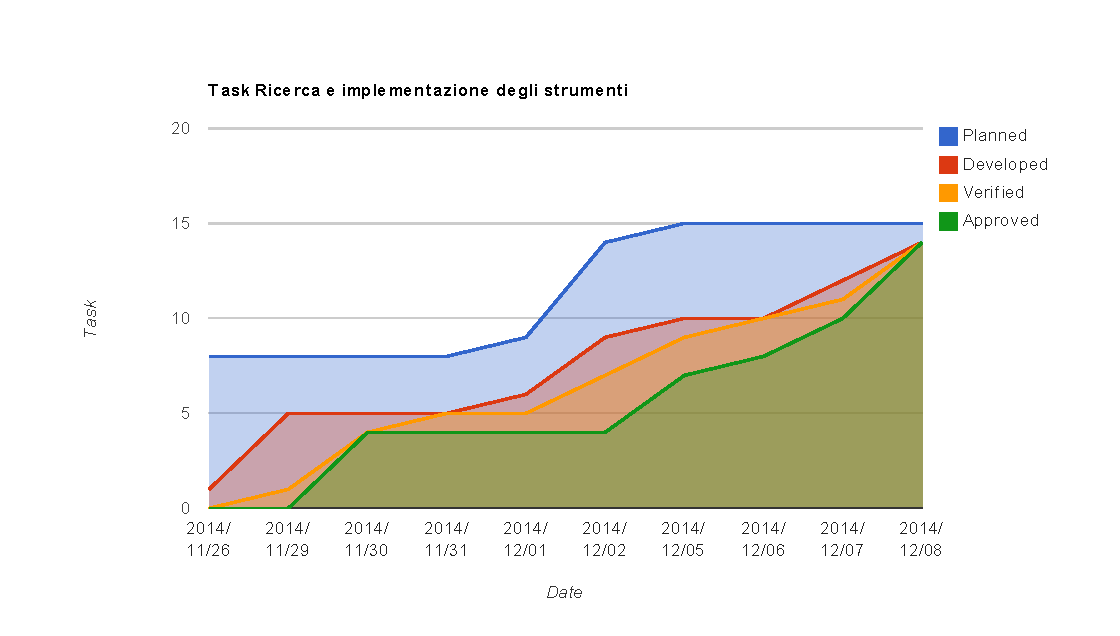
\includegraphics[scale=1]{images/Grafico_fase_1.pdf}}
				\caption{Grafico task Ricerca ed implementazione degli strumenti}
				\label{fig:taskfase1}
			\end{figure}
		\subsubsection{Documenti}
		Essendo in questa fase non presente ancora alcun documento, non è stato possibile verificarli e quindi avere dei valori da esporre. Per correttezza è stato comunque inserito il nome della fase.
	
	\subsection{Analisi dei requisiti}
		\subsubsection{Processi}
		La figura 4 rappresenta l'andamento dei task relativi a questa fase, si nota che dato l'inesperienza del gruppo e il tipo di fase in cui ci troviamo, inizialmente non ci sono molti task pianificati come ci si potrebbe aspettare in altre fasi. Il gruppo ha proseguito a pianificare pochi task alla volta fino al primo incontro con il proponente. Dal 2015/01/14 si osserva infatti un notevole picco inizialmente per i Planned ma poi anche per i Developed Verified e Approved. 
			\begin{figure}[htbp]
				\centering
				\centerline{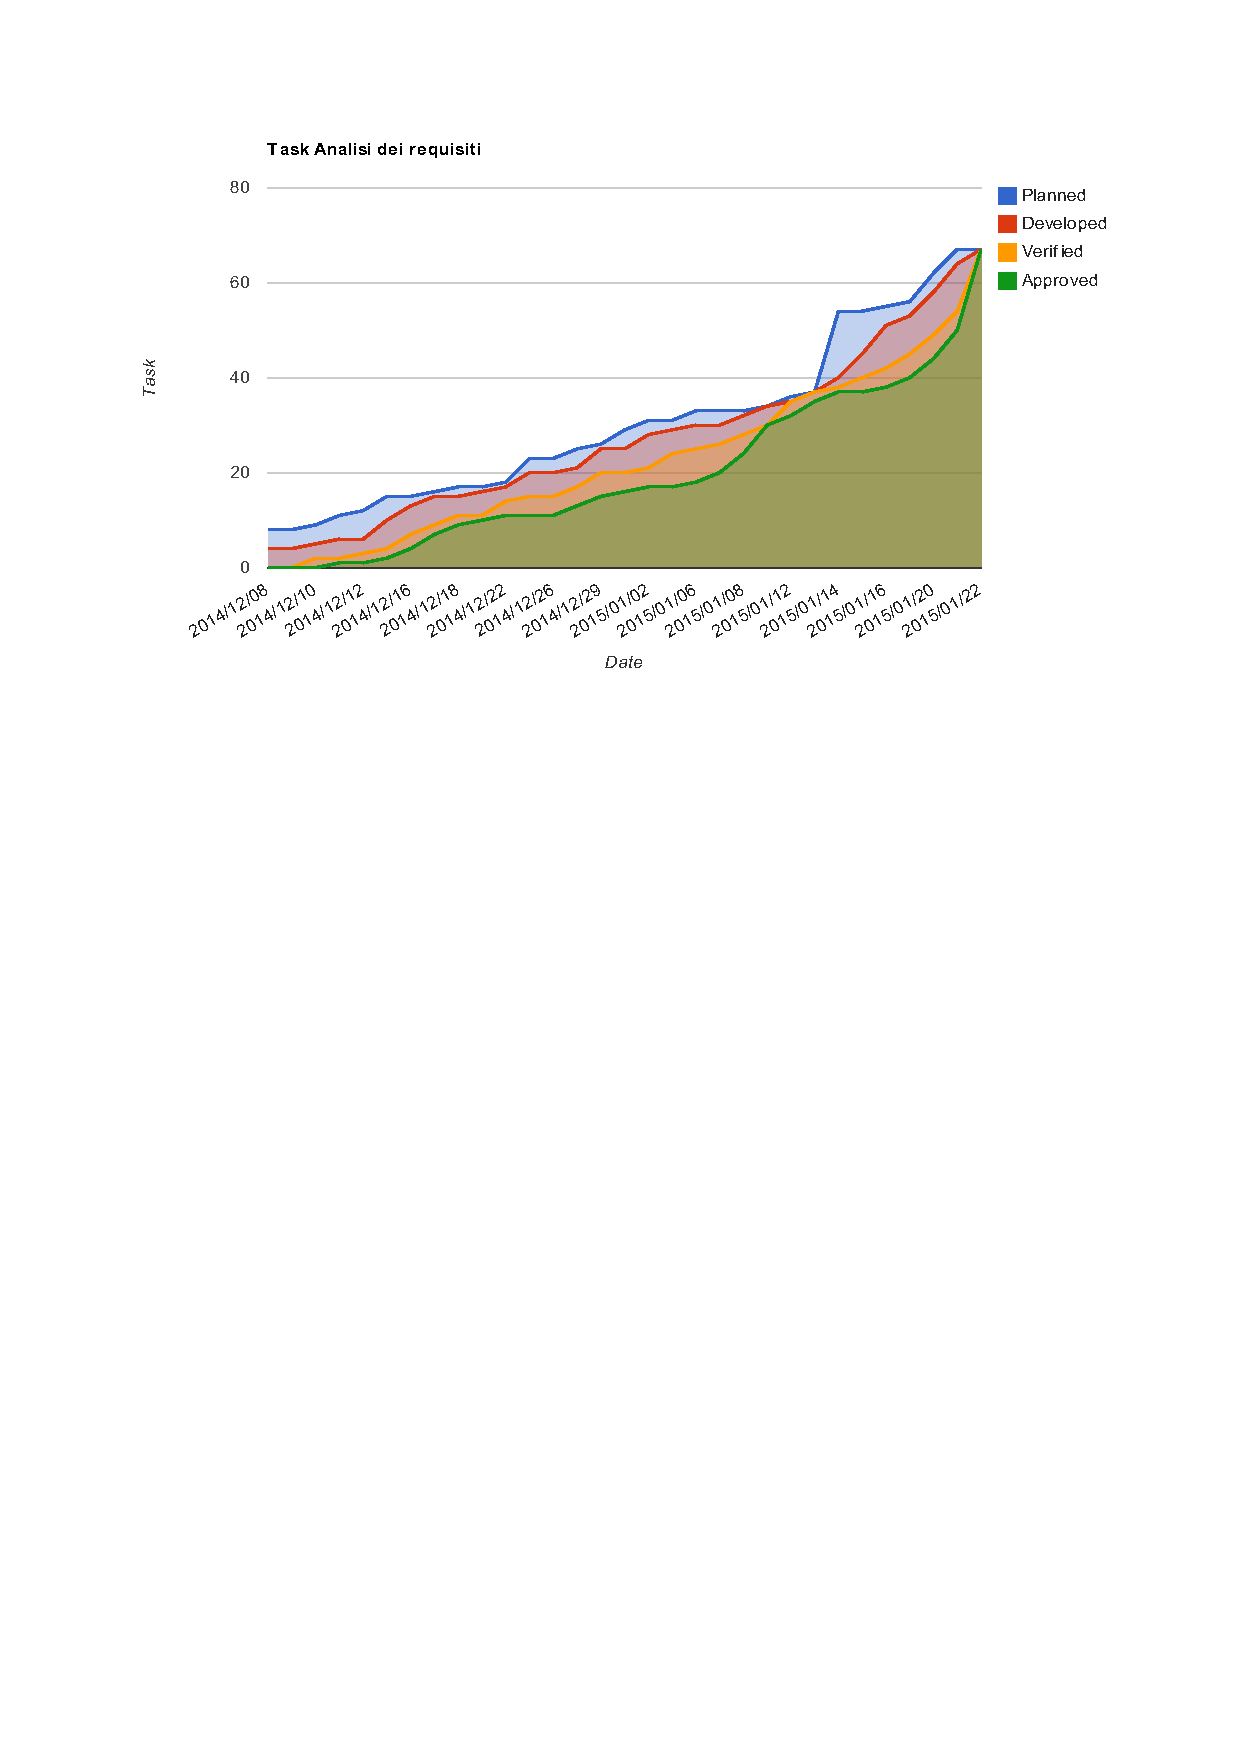
\includegraphics[scale=1]{images/Grafico_fase_2.pdf}}
				\caption{Grafico task Analisi dei requisiti}
				\label{fig:taskfase2}
			\end{figure}
	 	\subsubsection{Documenti}
	 	Vengono riportati i valori dell'indice di Gulpease relativi alla fase Analisi dei requisiti. Un documento va considerato accettabile solamente se rientra nelle metriche definite nella sezione.
		\begin{table}[!ht]
			\begin{center}
				\begin{tabularx}{0.9\textwidth}{|l|l|X|}
					\hline
					\textbf{Nome documento} & \textbf{Valore indice} & \textbf{Esito}\\
					\hline						
					\docNameVersionAdR & 56 & \textcolor{green}{Superato}\\
					\hline
					\docNameVersionGlo & 50 & \textcolor{green}{Superato}\\
					\hline					
					\docNameVersionNdP & 54 & \textcolor{green}{Superato}\\
					\hline					
					\docNameVersionPdP & 55 & \textcolor{green}{Superato}\\
					\hline					
					\docNameVersionPdQ & 55 & \textcolor{green}{Superato}\\
					\hline					
					\docNameVersionSdF & 48 & \textcolor{green}{Superato}\\
					\hline				
				\end{tabularx}
			\end{center}
			\caption{Risultati indice Gulpease}
		\end{table}
		\subsection{Analisi di dettaglio}
		\subsubsection{Processi}
		Inizialmente sono presenti molti task già pianificati questo anche perché la  riunione del team è stata fatta nel periodo iniziale della fase. Grazie a tale accorgimento è stato possibile pianificare con anticipo i task e quindi dare maggiore libertà in termini di tempistiche a coloro che dovevano completarli,  approvarli e verificarli.  \\
		Nel grafico si può notare che c'è un notevole aumento dei task Verified e Approved tra il 2015/02/05 e il 2015/02/06, i motivo e che il \roleProjectManager \ ha fissato la data di consegna di tutte le parti della presentazione il 2015/02/06. Il gruppo di conseguenza, ha cercato di rispettare al meglio la consegna, questo ha fatto si che ci fossero le giuste tempistiche per le prove della presentazione nonché l'integrazione con tutte le parti. Si osserva in oltre che non sono stati completati tutti i task pianificati, il motivo è che tutti i membri del gruppo negli ultimi giorni si sono impegnati a perfezionare la presentazione tralasciando in parte il lavoro da svolgere. Il non completamento di tutti i task andrà perciò ad appesantire la fase successiva nella quale bisognerà integrare anche questi task a quelli della fase.
		\begin{figure}[htbp]
				\centering
				\centerline{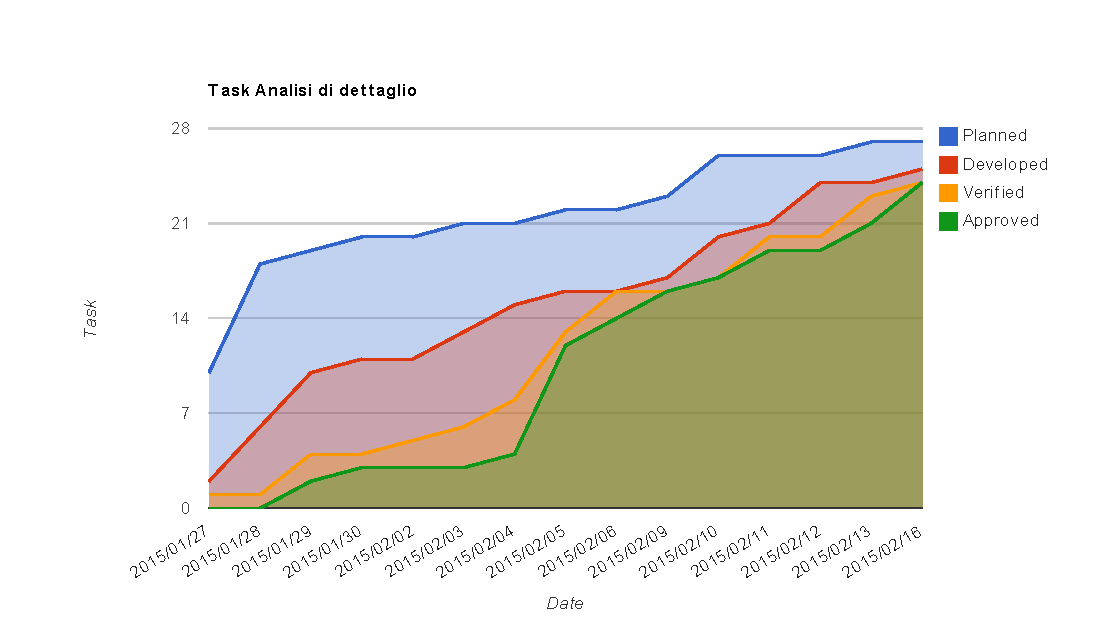
\includegraphics[scale=1]{images/Grafico_fase_3.pdf}}
				\caption{Grafico task Analisi di dettaglio}
				\label{fig:taskfase3}
			\end{figure}		
	 	\subsubsection{Documenti}
	 	Vengono riportati i valori dell'indice di Gulpease relativi alla fase Analisi di dettaglio. Un documento va considerato accettabile solamente se rientra nelle metriche definite nella sezione.
		\begin{table}[!ht]
			\begin{center}
				\begin{tabularx}{0.9\textwidth}{|l|l|X|}
					\hline
					\textbf{Nome documento} & \textbf{Valore indice} & \textbf{Esito}\\
					\hline						
					\docNameVersionAdR & ?? & \textcolor{green}{Superato}\\
					\hline
					\docNameVersionGlo & ?? & \textcolor{green}{Superato}\\
					\hline					
					\docNameVersionNdP & ?? & \textcolor{green}{Superato}\\
					\hline					
					\docNameVersionPdP & ?? & \textcolor{green}{Superato}\\
					\hline					
					\docNameVersionPdQ & ?? & \textcolor{green}{Superato}\\
					\hline					
					\docNameVersionSdF & ?? & \textcolor{green}{Superato}\\
					\hline				
				\end{tabularx}
			\end{center}
			\caption{Risultati indice Gulpease}
		\end{table}
		\subsection{Progettazione architetturale}
		\subsubsection{Processi}
		Visto il successo riscontrato nella fase precedente si è deciso di rendere una best practice la volontà di fissare una riunione nel primo periodo della fase per pianificare il più possibile e aver successivamente più tempo per il completamento, la verifica e l'approvazione. Nonostante quest'accorgimento il gruppo ha sforato la data pianificata di chiusura della fase che era il 2015/03/23, per finire ad approvare gli ultimi task il 2015/03/30. Il ritardo è stato dato in parte dal fatto che i membri del gruppo si sono scontrati con un nuovo linguaggio, e con nuovi software, questi hanno avuto bisogno di un apprendimento, attraverso studio e incontri col proponente, che è durato più del panificato. Si è scelto di estendere il grafico fino alla data di effettiva approvazione dell'ultimo task per dar maggior visibilità al way of working.
		\begin{figure}[htbp]
				\centering
				\centerline{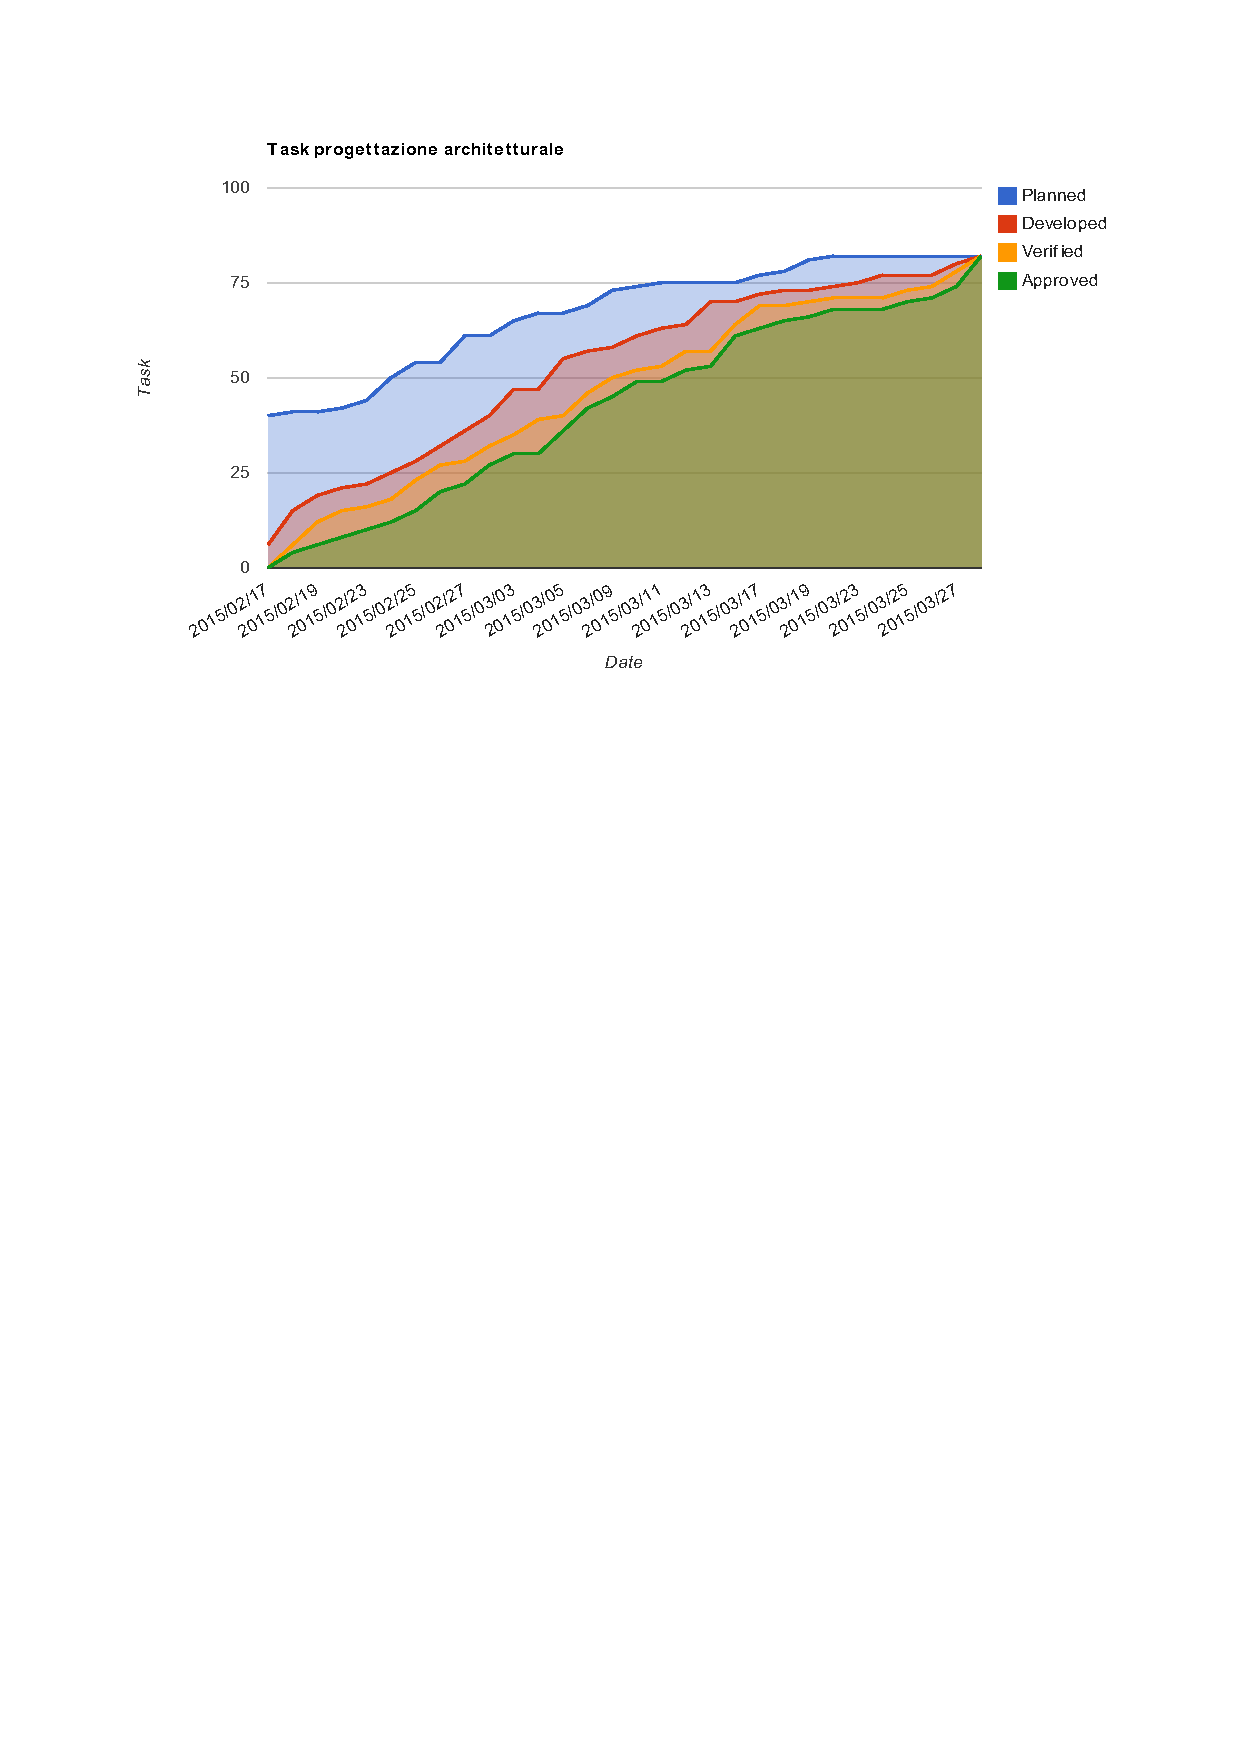
\includegraphics[scale=1]{images/Grafico_fase_4.pdf}}
				\caption{Grafico task Analisi di dettaglio}
				\label{fig:taskfase4}
			\end{figure}
	 	\subsubsection{Documenti}	 	
	 	Vengono riportati i valori dell'indice di Gulpease relativi alla fase Progettazione architetturale. Un documento va considerato accettabile solamente se rientra nelle metriche definite nella sezione.
		\begin{table}[!ht]
			\begin{center}
				\begin{tabularx}{0.9\textwidth}{|l|l|X|}
					\hline
					\textbf{Nome documento} & \textbf{Valore indice} & \textbf{Esito}\\
					\hline						
					\docNameVersionAdR & ?? & \textcolor{green}{Superato}\\
					\hline
					\docNameVersionGlo & ?? & \textcolor{green}{Superato}\\
					\hline					
					\docNameVersionNdP & ?? & \textcolor{green}{Superato}\\
					\hline					
					\docNameVersionPdP & ?? & \textcolor{green}{Superato}\\
					\hline					
					\docNameVersionPdQ & ?? & \textcolor{green}{Superato}\\
					\hline					
					\docNameVersionSdF & ?? & \textcolor{green}{Superato}\\
					\hline	
					\docNameVersionST & ?? & \textcolor{green}{Superato}\\
					\hline			
				\end{tabularx}
			\end{center}
			\caption{Risultati indice Gulpease}
		\end{table}s
	
\pagebreak